%! TEX program = xelatex
%! TEX encoding = UTF-8 Unicode

\documentclass[engineeringmaster]{hquThesis}
\usepackage{lineno}
\usepackage{amsmath,amsfonts,amssymb,textcomp,ulem}
\usepackage{booktabs,multirow,tabularx,float}
\usepackage{listings}
\lstset{
  breaklines,%自动换行
  columns=flexible,%不随便添加空格,只在已经有空格的地方添加空格,
}



\hypersetup{colorlinks=true,linkcolor=black,citecolor=black}
\begin{document}
\makecover
% NOTE: 正式文档请取消下面两行注释
% {
    \begin{center}
        \sffamily\fontsize{16pt}{25pt}\selectfont 学\hspace{8pt}位\hspace{8pt}论\hspace{8pt}文\hspace{8pt}答\hspace{8pt}辩\hspace{8pt}委\hspace{8pt}员\hspace{8pt}会\hspace{8pt}决\hspace{8pt}议
    \end{center}
} \vspace{32pt}
{
    \fontsize{14pt}{26pt}\selectfont
    \noindent\hspace{28pt}\rmfamily 根据《中华人民共和国学位条例》、《中华人民共和国学位条例暂行实 施办法》、《华侨大学学位授予工作细则》及《华侨大学研究生学位论文质 量监控与评阅答辩的管理规定》的规定,学位论文答辩委员会经充分交换意 见,对论文做出评价,并以无记名投票方式进行表决,同意该同学通过\degree 学位论文答辩,同意授予\degree 学位。\par
    \vspace{192pt}
    \noindent\flushright 答辩委员会(主席签字):\underline{\hspace{156pt}}\vspace{14pt} \par
    \noindent\flushright 答辩时间:\underline{\hspace{60pt}}年\underline{\hspace{25pt}}月\underline{\hspace{25pt}}日 \par
}

% \noindent\fbox{%
    \parbox{14.3cm}{
    \vspace{24pt}\begin{center}\sffamily\fontsize{16pt}{\baselineskip}\selectfont 学位论文独创性声明\end{center}\vspace{18pt}
    \hspace{28pt}\declarationfont\fontsize{14pt}{28pt}\selectfont
    本人声明兹呈交的学位论文是本人在导师指导下完成的研究成果。论文写作中不包含其他人已经发表或撰写过的研究内容,如参考他人或集体的科研成果,均在论文中以明确的方式说明。本人依法享有和承担由此论文所产生的权利和责任。\par
    \vspace{28pt}\hspace{28pt} 论文作者签名:\underline{\hspace{112pt}}\hspace{7pt}签名日期:\underline{\hspace{77pt}}\par\vspace{7pt}
    }%
}
\par
\vspace{44pt}
\noindent\framebox[\linewidth]{
    \parbox{14.3cm}{
    \vspace{24pt}\begin{center}\sffamily\fontsize{16pt}{\baselineskip}\selectfont 学位论文版权使用授权声明\par\end{center}\vspace{18pt}
    \hspace{28pt}\declarationfont\fontsize{14pt}{28pt}\selectfont 
    本人同意授权华侨大学有权保留并向国家机关或机构送交学位论文的复印件和电子版,允许学位论文被查阅和借阅。本人授权华侨大学可以将本学位论文的全部内容或部分内容编入有关数据库进行检索,可以采用影印、缩印或扫描等复制手段保存和汇编本学位论文。\par\vspace{28pt}
    \hspace{28pt}论文作者签名:\underline{\hspace{84pt}}\hspace{7pt}指导老师签名:\underline{\hspace{84pt}}\par
    \hspace{28pt}签\hspace{7pt}名\hspace{7pt}日\hspace{7pt}期:\underline{\hspace{91pt}}\hspace{7pt}签\hspace{7pt}名\hspace{7pt}日\hspace{7pt}期:\underline{\hspace{91pt}}\par\vspace{7pt}
    }
}


\frontmatter{
    % TODO: 设置摘要
\begin{abstract}
    测试摘大大范德萨范德萨范德萨发大水范德萨范德萨范德萨范德萨范德萨范德萨范德萨的撒范德萨范德萨范德萨范德萨范德萨范德萨发大顺丰。
\end{abstract}
\keywords{关键词1;关键词2;关键词3;关键词4;关键词5}
\begin{abstractEn}
fdsa
\end{abstractEn}
\keywordsEn{keyword1; keyword2; keyword3; keyword4; keyword5; keyword6; keyword7; keyword8}

    \tableofcontents
}

\mainmatter
\chapter{前期准备}
\section{封面关键字设置}
\section{Git相关}
使用fork建仓,
网页链接:\href{https://docs.github.com/en/repositories/creating-and-managing-repositories/creating-a-template-repository}{建仓步骤}

\section{VS code配置}
\subsection*{建立Tmp文件:}
在VSCode中修改LaTex WorkShop配置以指定输出目录,在json中添加以下代码(将编译过程中不必要的文件存储在Tmp文件中):

以下是在json文件中关于Latex的设置内容:详细介绍链接\href{https://zhuanlan.zhihu.com/p/166523064}{vsocde中的Latex配置}
\begin{lstlisting}
    // ======================== LaTeX 设置 BEGIN  ========================

    // ======================== LaTeX 设置 END ========================
\end{lstlisting}

\subsection*{LaTeX workshop: }

正向搜索(forward research)从代码处定位至PDF文档处:Ctrl+alt+j

反向搜索(inverse research)从PDF文档准确定位至LaTeX代码处:Ctrl+鼠标左键

网页链接:\href{https://github.com/James-Yu/LaTeX-Workshop/wiki/View#synctex}{正反向搜索介绍}
\subsection*{Git Graph}
点击左侧源代码管理插件-点击左上角View Git Graph(git log)-查看修改记录

\subsection*{Todo Tree}
帮助管理项目中的TODO注释和其他标记

网页链接:\href{https://blog.csdn.net/m0_37586991/article/details/104239568}{Todo Tree安装步骤}

\subsection*{Zotero LaTeX}
Zotero管理参考文献
\section{文件、label 命名规则}
Latex路径中文件只允许以英文命名

\subsection*{公式}
\begin{lstlisting}
    \label{CH_name}{formula_name}
\end{lstlisting}

\subsection*{图}
\begin{lstlisting}
    \label{CH_name}{fig_name}
\end{lstlisting}

\subsection*{表}
\begin{lstlisting}
    \label{CH_name}{table_name}
\end{lstlisting}


\chapter{图表设置}
\subsection*{单张}
\begin{figure}[H]
    \centering
    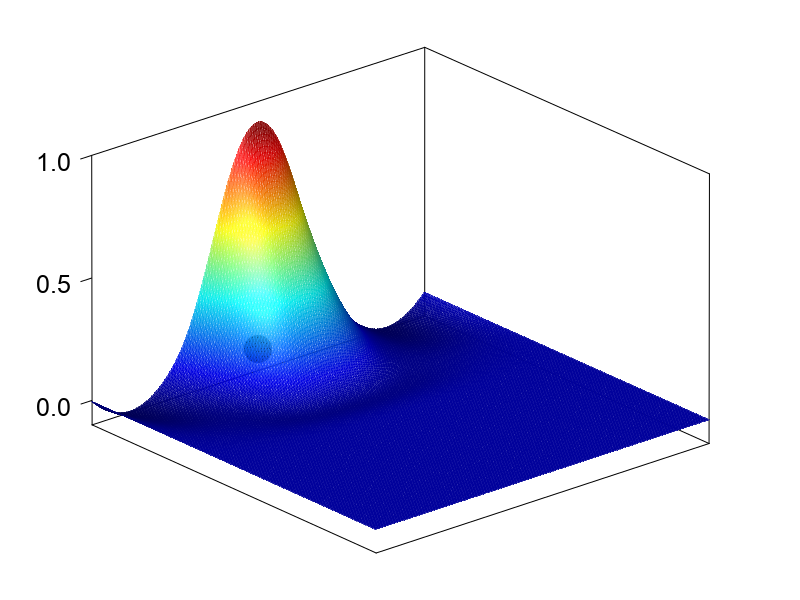
\includegraphics[scale=0.4]{figure/1.png}
\caption{\centering{边界点处无网格形函数}}
\label{CHGraphsettings_fig1_meshfree}
\end{figure}
单张图片Latex代码
\begin{lstlisting}
\begin{figure}[H]-放置位置
\centering-居中
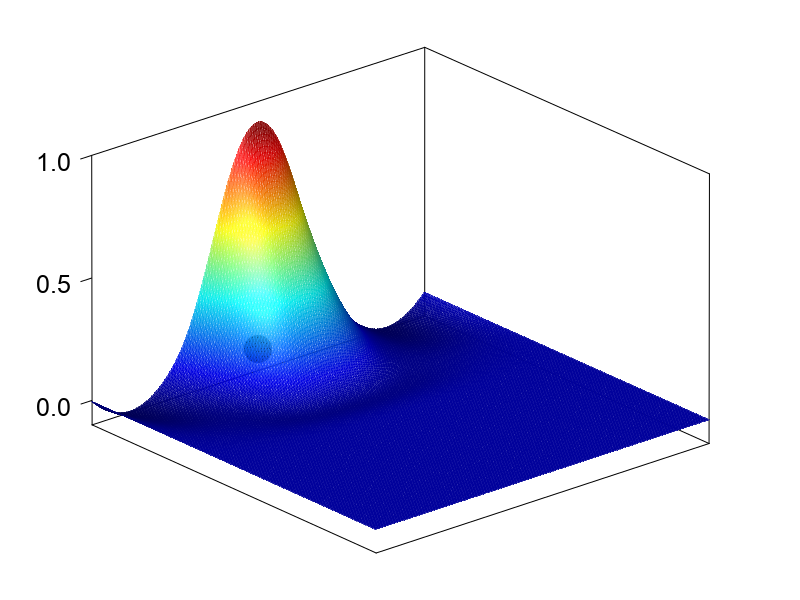
\includegraphics[scale=0.4]{figure/1.png}-大小、图片路径
\caption{\centering{边界点处无网格形函数}}-图名
\label{CHGraphsettings_fig1_meshfree}-命名
\end{figure}
\end{lstlisting}
\subsection*{并排}
\begin{figure}[H]
    \centering
    \begin{subcaptiongroup}
    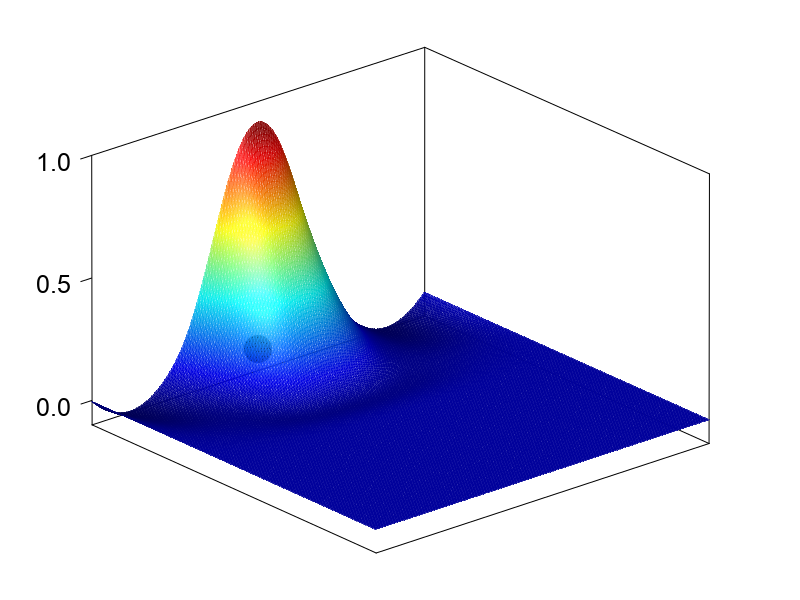
\includegraphics[width=0.49\textwidth]{figure/1.png}
    \phantomcaption\label{1}
    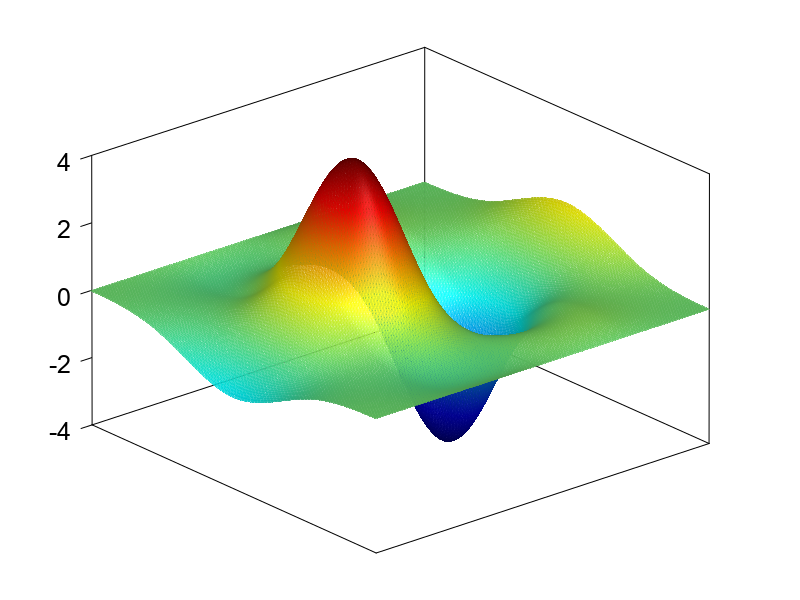
\includegraphics[width=0.49\textwidth]{figure/2.png}
    \phantomcaption\label{2}
    \end{subcaptiongroup}
\caption{\centering{无网格形函数:\subref{1}边界点;\subref{2}中心点}}
% NOTE:遇到图名过长需要换行的编写:
% \caption{\centering{标题:\protect\linebreak \subref{xxx} 小标题1;\subref{xx} 小标题2;\subref{xxx}小标题3;\subref{xxx} 小标题4}}
\label{CHGraphsettings_fig2_meshfree}
\end{figure}
并排图片Latex代码
\begin{lstlisting}
\begin{figure}[H]
\centering
\begin{subcaptiongroup}
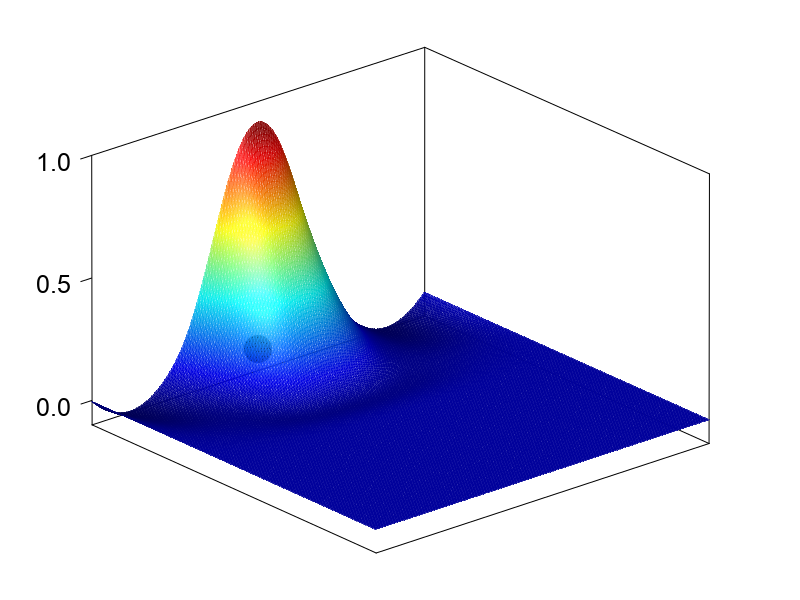
\includegraphics[width=0.49\textwidth]{figure/1.png}
\phantomcaption\label{1}
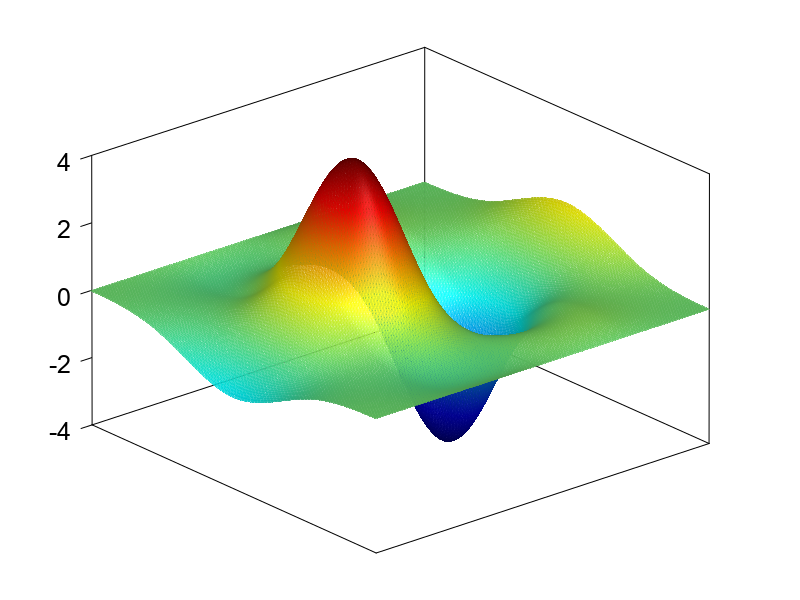
\includegraphics[width=0.49\textwidth]{figure/2.png}
\phantomcaption\label{2}
\end{subcaptiongroup}
\caption{\centering{无网格形函数:\subref{1}边界点;\subref{2}中心点}}
\end{lstlisting}
图\ref{CHGraphsettings_fig1_meshfree}、\ref{CHGraphsettings_fig2_meshfree}分别表示边界点处和内部节点处的无网格形函数图。

\subsection*{表格式图片}
\begin{figure}[H]
    \centering
    \begin{tabular}{cccc}
    $\quad$&$p=2$&$p=2$&$p=2$\\
    边界点&\begin{subcaptiongroup}\raisebox{-0.5\height}{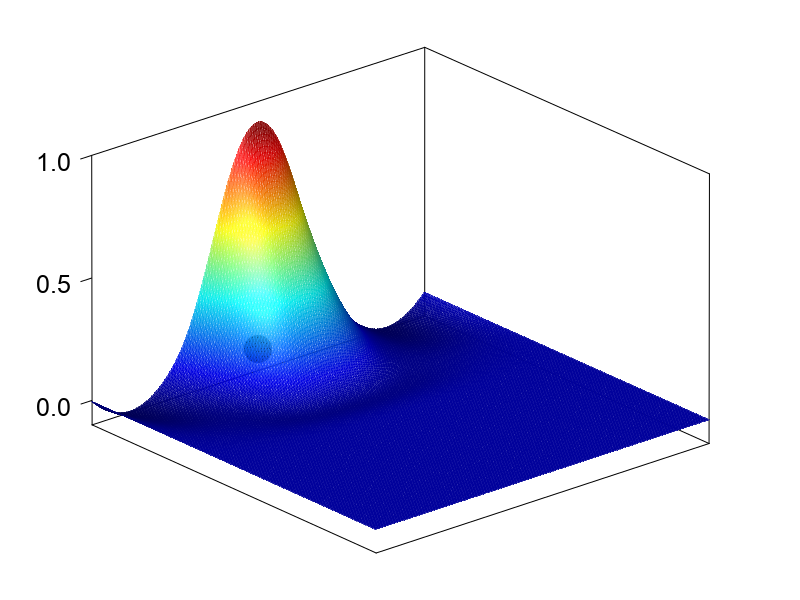
\includegraphics[width=0.3\textwidth]{figure/1.png}}\end{subcaptiongroup}
    &\begin{subcaptiongroup}\raisebox{-0.5\height}{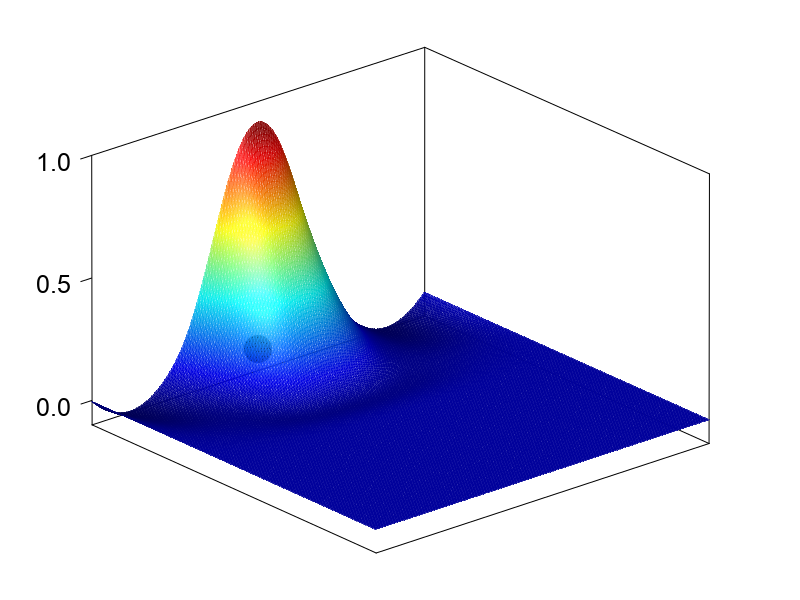
\includegraphics[width=0.3\textwidth]{figure/1.png}}\end{subcaptiongroup}
    &\begin{subcaptiongroup}\raisebox{-0.5\height}{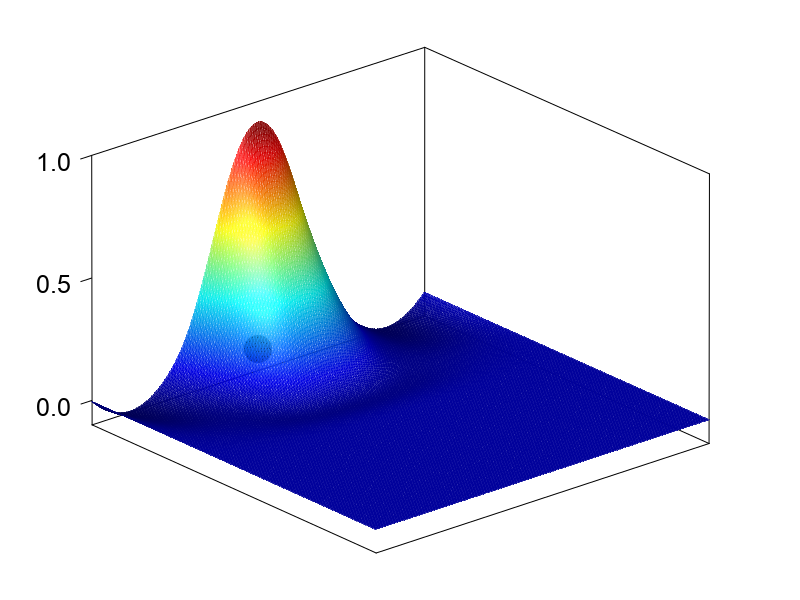
\includegraphics[width=0.3\textwidth]{figure/1.png}}\end{subcaptiongroup}\\
    中心点&\begin{subcaptiongroup}\raisebox{-0.5\height}{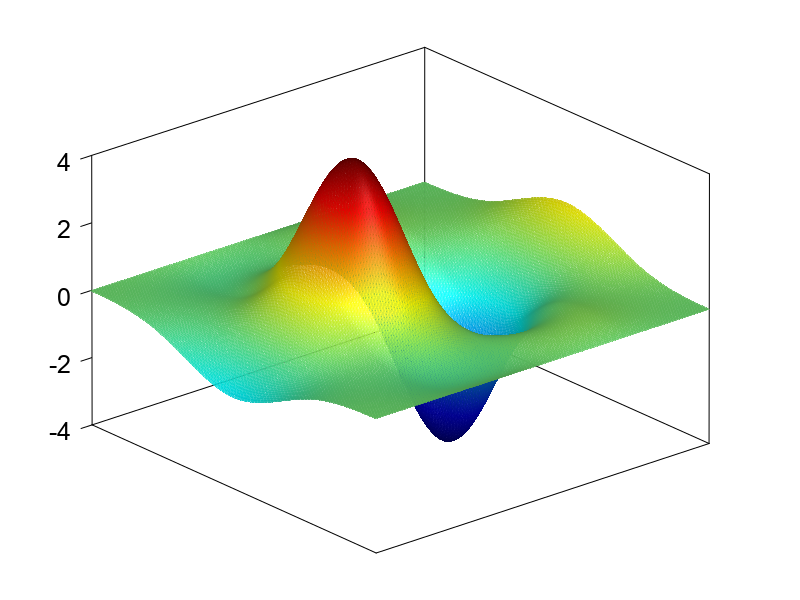
\includegraphics[width=0.3\textwidth]{figure/2.png}}\end{subcaptiongroup}
    &\begin{subcaptiongroup}\raisebox{-0.5\height}{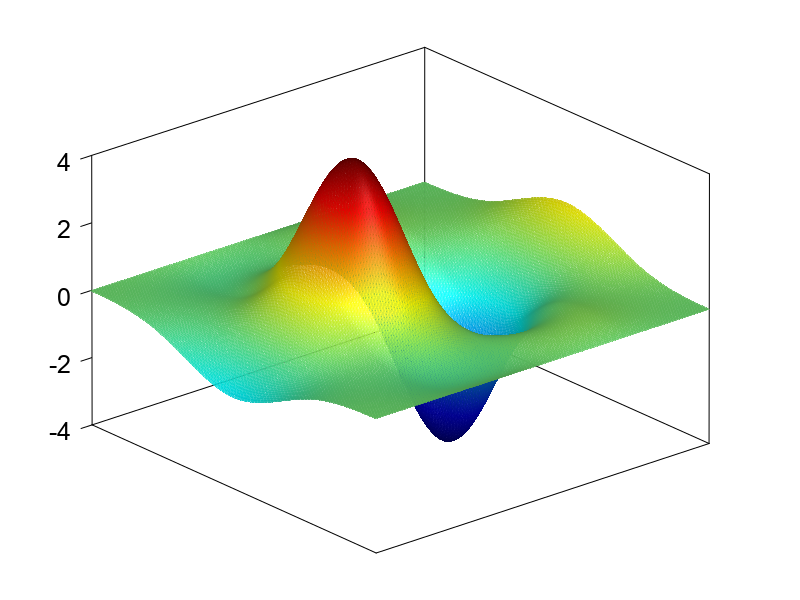
\includegraphics[width=0.3\textwidth]{figure/2.png}}\end{subcaptiongroup}
    &\begin{subcaptiongroup}\raisebox{-0.5\height}{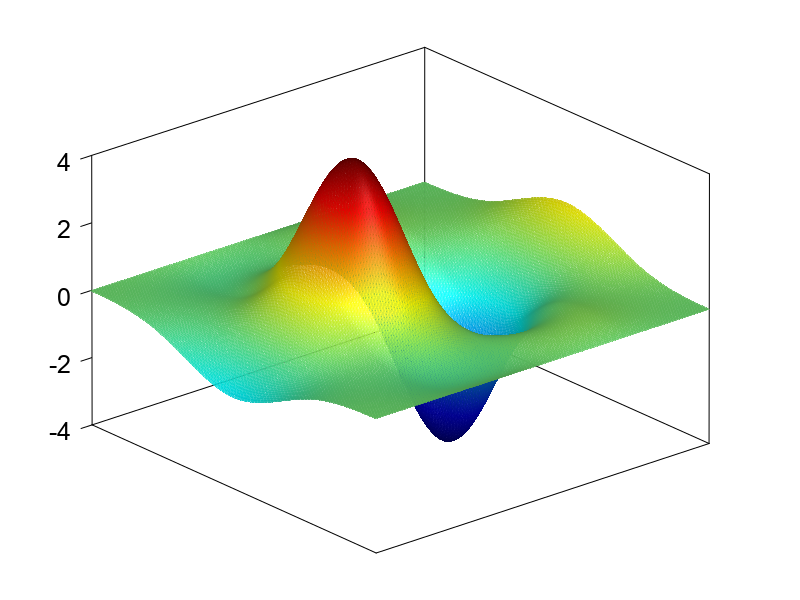
\includegraphics[width=0.3\textwidth]{figure/2.png}}\end{subcaptiongroup}\\
    \end{tabular}
    \caption{\textbf{二维边界点与内部节点无网格形函数图}}\label{CHGraphsettings_fig3_meshfree}
    \end{figure}

表格式图片Latex代码
\begin{lstlisting}
\begin{figure}[H]
\centering
\begin{tabular}{cccc}
$\quad$&$p=2$&$p=2$&$p=2$\\
边界点&\begin{subcaptiongroup}\raisebox{-0.5\height}{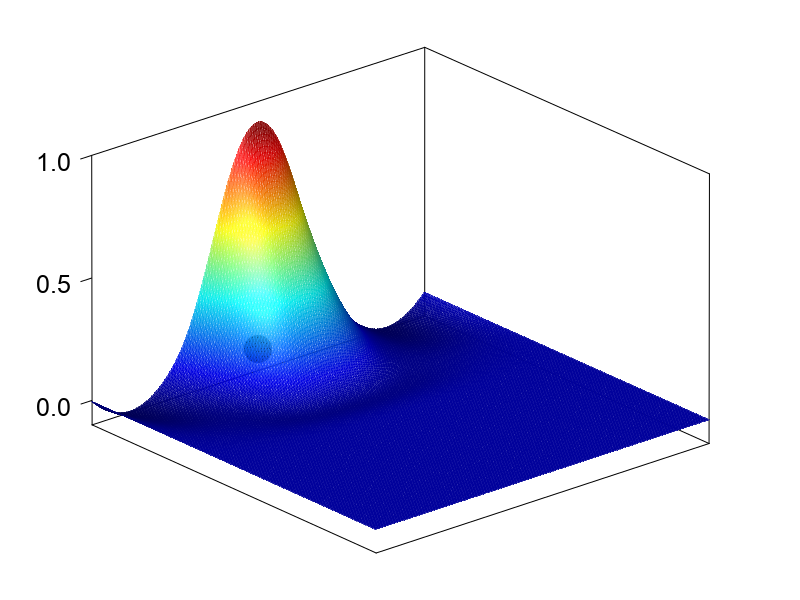
\includegraphics[width=0.3\textwidth]{figure/1.png}}\end{subcaptiongroup}
&\begin{subcaptiongroup}\raisebox{-0.5\height}{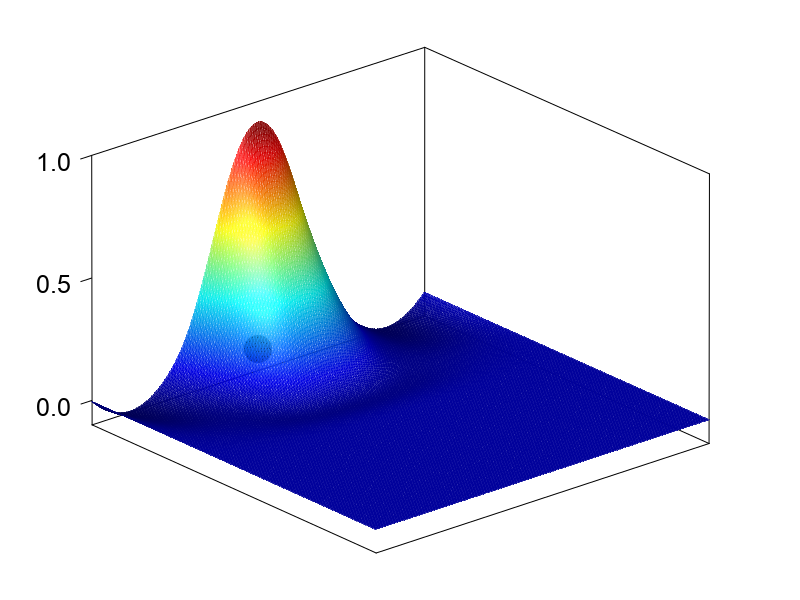
\includegraphics[width=0.3\textwidth]{figure/1.png}}\end{subcaptiongroup}
&\begin{subcaptiongroup}\raisebox{-0.5\height}{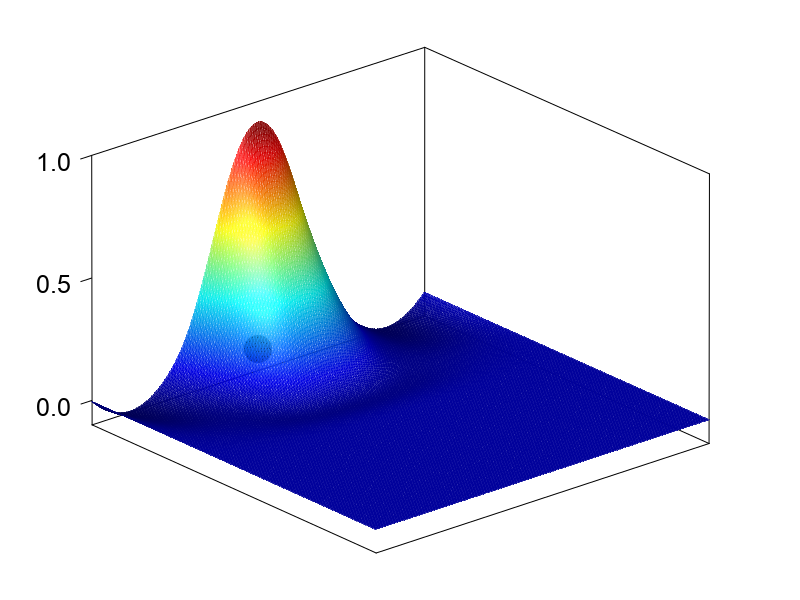
\includegraphics[width=0.3\textwidth]{figure/1.png}}\end{subcaptiongroup}\\
中心点&\begin{subcaptiongroup}\raisebox{-0.5\height}{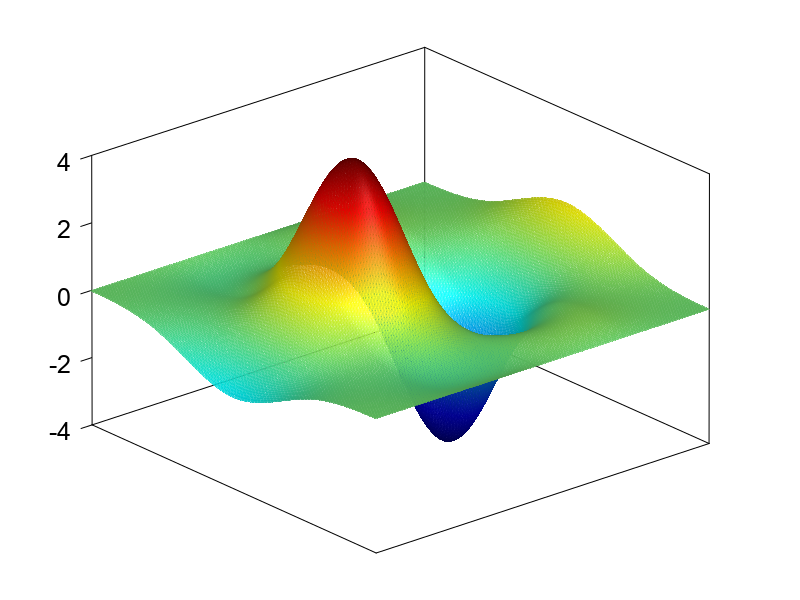
\includegraphics[width=0.3\textwidth]{figure/2.png}}\end{subcaptiongroup}
&\begin{subcaptiongroup}\raisebox{-0.5\height}{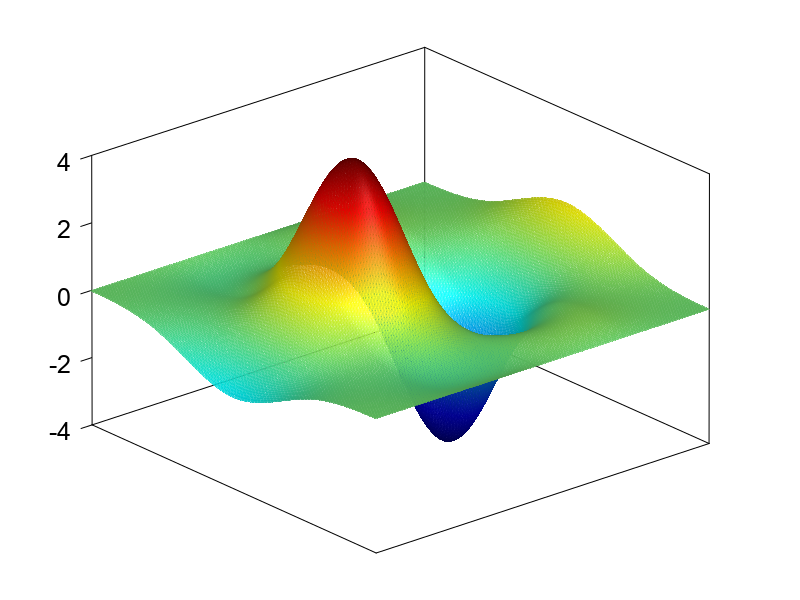
\includegraphics[width=0.3\textwidth]{figure/2.png}}\end{subcaptiongroup}
&\begin{subcaptiongroup}\raisebox{-0.5\height}{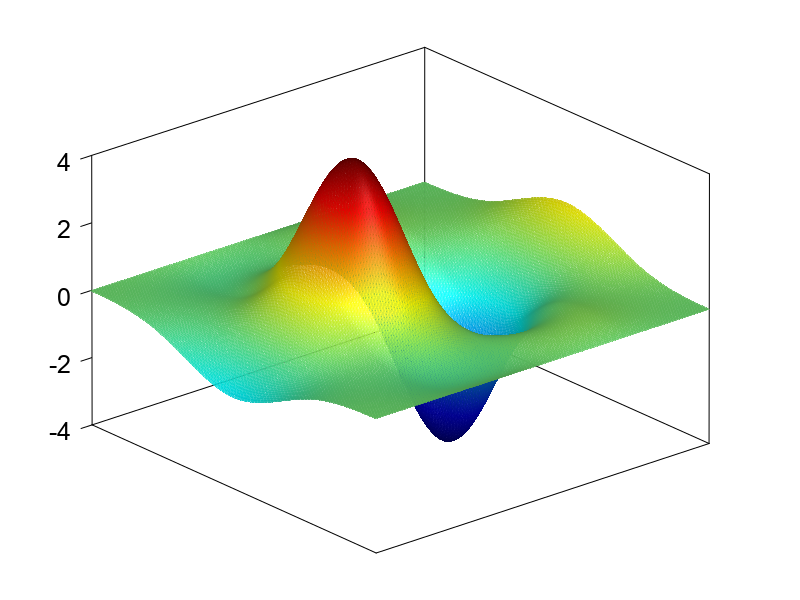
\includegraphics[width=0.3\textwidth]{figure/2.png}}\end{subcaptiongroup}\\
\end{tabular}
\caption{\textbf{二维边界点与内部节点无网格形函数图}}\label{CHGraphsettings_fig3_meshfree}
\end{figure}     
\end{lstlisting}

\subsection*{三线表}
\begin{table}[H]
    \caption{\textbf{三次基函数无网格法分片实验结果}}
    \centering\label{CHGraphsettings_table_cubic}
    \begin{tabular}{lcccc}
       \toprule
    & \multicolumn{2}{c}{二次分片实验} & \multicolumn{2}{c}{三次分片实验} \\ \cline{2-5}
       &$L_2$-Error$\quad$&$H_1$-Error&$L_2$-Error$\quad$&$H_1$-Error\\
       \midrule
      RKGSI-Penalty&$1.4\times10^{-7}$&$2.1\times10^{-6}$&$2.0\times10^{-7}$&$2.7\times10^{-6}$\\
      RKGSI-LM&$3.0\times10^{-4}$&$9.8\times10^{-3}$&$4.2\times10^{-4}$&$9.8\times10^{-3}$\\
      RKGSI-Nitsche&$3.6\times10^{-15}$&$1.0\times10^{-13}$&$4.6\times10^{-15}$&$9.5\times10^{-14}$\\
      RKGSI-HR&$3.1\times10^{-15}$&$1.0\times10^{-13}$&$3.5\times10^{-15}$&$7.4\times10^{-14}$\\
       \bottomrule
    \end{tabular}
    \end{table}
三线表Latex代码
\begin{lstlisting}
\begin{table}[H]
\caption{\textbf{三次基函数无网格法分片实验结果}}
\centering\label{CHGraphsettings_table_cubic}
\begin{tabular}{lcccc}
\toprule
& \multicolumn{2}{c}{二次分片实验} & \multicolumn{2}{c}{三次分片实验} \\ \cline{2-5}
&$L_2$-Error$\quad$&$H_1$-Error&$L_2$-Error$\quad$&$H_1$-Error\\
\midrule
RKGSI-Penalty&$1.4\times10^{-7}$&$2.1\times10^{-6}$&$2.0\times10^{-7}$&$2.7\times10^{-6}$\\
RKGSI-LM&$3.0\times10^{-4}$&$9.8\times10^{-3}$&$4.2\times10^{-4}$&$9.8\times10^{-3}$\\
RKGSI-Nitsche&$3.6\times10^{-15}$&$1.0\times10^{-13}$&$4.6\times10^{-15}$&$9.5\times10^{-14}$\\
RKGSI-HR&$3.1\times10^{-15}$&$1.0\times10^{-13}$&$3.5\times10^{-15}$&$7.4\times10^{-14}$\\
\bottomrule
\end{tabular}
\end{table}    
\end{lstlisting}
表\ref{CHGraphsettings_table_cubic}为三次基函数无网格法的分片试验结果。

\chapter{使用Zotero管理参考文献}
1.下载附件:Better BibTex
链接:\href{https://zhuanlan.zhihu.com/p/621145900}{Better BibTex安装步骤}

2.新建分类建立文件库:references

3.右击该文件库-选择导出分类-以Better BibTex形式导出条目

4.导出条目至与Latex文件相同路径

5.在主文件(ef:main.tex)中添加:
\begin{lstlisting}
\begin{document}
    .....
    \bibliography{references}--导出文献的文件名
    .....
\end{document}
\end{lstlisting}
eg:基于赫林格-赖斯纳原理的变分一致型伽辽金无网格法\cite{Wu2022,wu2023}相较于传统的本质边界条件施加方法能够有效提高计算精度和计算效率。

Latex代码

\begin{lstlisting}
eg:基于赫林格-赖斯纳原理的变分一致型伽辽金无网格法\cite{Wu2022,wu2023}相较于传统的本质边界条件施加方法能够有效提高计算精度和计算效率。
\end{lstlisting}

\chapter{\LaTeX 部分所需包介绍}


编写公式-\{amsmath,amsfonts,amssymb,textcomp,ulem\}

绘制表格-\{booktabs,multirow,tabularx,float\}

书写代码-\{listings\}

代码块设置
\begin{lstlisting}
\lstset{
  breaklines,%自动换行
  columns=flexible,%不随便添加空格,只在已经有空格的地方添加空格,
}
\end{lstlisting}

设置PDF文档中超链接的颜色
\begin{lstlisting}
\hypersetup{colorlinks=true,linkcolor=black,citecolor=black}
\end{lstlisting}



% NOTE 毕业论文致谢部分
% \begin{acknowledgements}
感谢
\end{acknowledgements}

\appendix
\chapter{附录}
附录章节前添加如下代码
\begin{lstlisting}
    \appendix
\end{lstlisting}


\chapter{参考格式}
\begin{lstlisting}

\documentclass[engineeringmaster]{hquThesis}-hquThesis是模板文件,包含文本格式,字体设置,文献格式.....
\usepackage{amsmath,amsfonts,amssymb,textcomp}-公式所需
\usepackage{booktabs,multirow,tabularx,float}-表格所需
\hypersetup{colorlinks=true,linkcolor=black,citecolor=black}-设置超链接格式
\titleZh{XXX}-中文标题
\titleEn{XXX}-英文标题
\id{}-学号
\authorZh{XXX}-作者姓名
\supervisorZh{XXX}{XXX}-指导教师+职称
\cosupervisorZh{XXX}{XXX}-合作教师+职称
\practicevisorZh{XXX}{XXX}-实践教师+职称
\departmentZh{土木工程学院}
\fieldZh{结构体系创新与工程应用}
\majortype{工程硕士}
\major{土木水利}
\coverdate{二〇二四年三月XX日}
-封面设置
\begin{document}-正文开始

\makecover
{
    \begin{center}
        \sffamily\fontsize{16pt}{25pt}\selectfont 学\hspace{8pt}位\hspace{8pt}论\hspace{8pt}文\hspace{8pt}答\hspace{8pt}辩\hspace{8pt}委\hspace{8pt}员\hspace{8pt}会\hspace{8pt}决\hspace{8pt}议
    \end{center}
} \vspace{32pt}
{
    \fontsize{14pt}{26pt}\selectfont
    \noindent\hspace{28pt}\rmfamily 根据《中华人民共和国学位条例》、《中华人民共和国学位条例暂行实 施办法》、《华侨大学学位授予工作细则》及《华侨大学研究生学位论文质 量监控与评阅答辩的管理规定》的规定,学位论文答辩委员会经充分交换意 见,对论文做出评价,并以无记名投票方式进行表决,同意该同学通过\degree 学位论文答辩,同意授予\degree 学位。\par
    \vspace{192pt}
    \noindent\flushright 答辩委员会(主席签字):\underline{\hspace{156pt}}\vspace{14pt} \par
    \noindent\flushright 答辩时间:\underline{\hspace{60pt}}年\underline{\hspace{25pt}}月\underline{\hspace{25pt}}日 \par
}
-答辩委员会
\noindent\fbox{%
    \parbox{14.3cm}{
    \vspace{24pt}\begin{center}\sffamily\fontsize{16pt}{\baselineskip}\selectfont 学位论文独创性声明\end{center}\vspace{18pt}
    \hspace{28pt}\declarationfont\fontsize{14pt}{28pt}\selectfont
    本人声明兹呈交的学位论文是本人在导师指导下完成的研究成果。论文写作中不包含其他人已经发表或撰写过的研究内容,如参考他人或集体的科研成果,均在论文中以明确的方式说明。本人依法享有和承担由此论文所产生的权利和责任。\par
    \vspace{28pt}\hspace{28pt} 论文作者签名:\underline{\hspace{112pt}}\hspace{7pt}签名日期:\underline{\hspace{77pt}}\par\vspace{7pt}
    }%
}
\par
\vspace{44pt}
\noindent\framebox[\linewidth]{
    \parbox{14.3cm}{
    \vspace{24pt}\begin{center}\sffamily\fontsize{16pt}{\baselineskip}\selectfont 学位论文版权使用授权声明\par\end{center}\vspace{18pt}
    \hspace{28pt}\declarationfont\fontsize{14pt}{28pt}\selectfont 
    本人同意授权华侨大学有权保留并向国家机关或机构送交学位论文的复印件和电子版,允许学位论文被查阅和借阅。本人授权华侨大学可以将本学位论文的全部内容或部分内容编入有关数据库进行检索,可以采用影印、缩印或扫描等复制手段保存和汇编本学位论文。\par\vspace{28pt}
    \hspace{28pt}论文作者签名:\underline{\hspace{84pt}}\hspace{7pt}指导老师签名:\underline{\hspace{84pt}}\par
    \hspace{28pt}签\hspace{7pt}名\hspace{7pt}日\hspace{7pt}期:\underline{\hspace{91pt}}\hspace{7pt}签\hspace{7pt}名\hspace{7pt}日\hspace{7pt}期:\underline{\hspace{91pt}}\par\vspace{7pt}
    }
}
-独创性说明
\frontmatter
% TODO: 设置摘要
\begin{abstract}
    测试摘大大范德萨范德萨范德萨发大水范德萨范德萨范德萨范德萨范德萨范德萨范德萨的撒范德萨范德萨范德萨范德萨范德萨范德萨发大顺丰。
\end{abstract}
\keywords{关键词1;关键词2;关键词3;关键词4;关键词5}
\begin{abstractEn}
fdsa
\end{abstractEn}
\keywordsEn{keyword1; keyword2; keyword3; keyword4; keyword5; keyword6; keyword7; keyword8}
-摘要
\tableofcontents
\mainmatter
\include{Introduction}-正文章节
\include{XXX}
\include{XXXX}
\backmatter-页眉另起设置
\bibliography{references}-引用参考文献条目(.bib)
\begin{acknowledgements}
感谢
\end{acknowledgements}
-致谢
\appendix-附录部分
\include{appendixA}-附录章节
\include{appendixB}-附录章节
\begin{cv}
    \section*{个人简历}
    XXX,女,汉族,XXXX年XX月XX日出生,XX省XXX人。

    XXXX年XX月毕业于XXXX学校XXXX专业,获得工学学士学位。

    XXXX年XX月至今就读于华侨大学土木工程学院土木水利专业,攻读工学硕士学位。
    \section*{在学期间发表的论文}
    \begin{enumerate}[{[1]}]
        \item 吴俊超, 邓俊俊, 王家睿, 等. 伽辽金型无网格法的数值积分方法[J]. 固体力学学报, 2016, 3(37): 208-233. 
        \item 吴俊超, 邓俊俊, 王家睿, 等. 伽辽金型无网格法的数值积分方法[J]. 固体力学学报, 2016, 3(37): 208-233. 
    \end{enumerate}
\end{cv}
-个人简历

\end{document}-结束正文
\end{lstlisting}


\backmatter


\bibliography{references}

% NOTE 毕业论文个人简历部分
% \begin{cv}
    \section*{个人简历}
    XXX,女,汉族,XXXX年XX月XX日出生,XX省XXX人。

    XXXX年XX月毕业于XXXX学校XXXX专业,获得工学学士学位。

    XXXX年XX月至今就读于华侨大学土木工程学院土木水利专业,攻读工学硕士学位。
    \section*{在学期间发表的论文}
    \begin{enumerate}[{[1]}]
        \item 吴俊超, 邓俊俊, 王家睿, 等. 伽辽金型无网格法的数值积分方法[J]. 固体力学学报, 2016, 3(37): 208-233. 
        \item 吴俊超, 邓俊俊, 王家睿, 等. 伽辽金型无网格法的数值积分方法[J]. 固体力学学报, 2016, 3(37): 208-233. 
    \end{enumerate}
\end{cv}


\end{document}
